\documentclass[spanish, a4paper]{article}

\usepackage{ulem}
\hoffset=-2cm \voffset=-2.5cm
\parskip=0.5cm
\topmargin 2cm

\textwidth 16cm
\textheight 24cm

\usepackage{caratula}
\usepackage[spanish]{babel}
\usepackage[utf8]{inputenc}
%\usepackage[latin1]{inputenc}
\usepackage{fancyhdr} %header lindo
\usepackage{listingsutf8}
\usepackage{pdfpages} %incluir pdf


\usepackage{caption}
\usepackage{subcaption}

\providecommand{\keywords}[1]{\textbf{\textit{Palabras Clave ---}} \textit{#1}}

\usepackage{color}

\definecolor{dkgreen}{rgb}{0,0.6,0}
\definecolor{gray}{rgb}{0.5,0.5,0.5}
\definecolor{mauve}{rgb}{0.58,0,0.82}

\lstset{inputencoding=utf8/latin1}
\lstset{
  frame=none,
  xleftmargin=0.1in,
  stepnumber=1,
  numbers=left,
%  numbersep=5pt,
  numberstyle=\ttfamily\tiny\color[gray]{0.3},
  belowcaptionskip=\bigskipamount,
  captionpos=b,
  escapeinside={*'}{'*},
%  language=Prolog,
  tabsize=1,
%  emphstyle={\bf},
%  commentstyle=\it,
%  stringstyle=\mdseries\rmfamily,
  showspaces=false,
  breaklines=true,
%  keywordstyle=\bfseries\rmfamily,
%  columns=flexible,
%  basicstyle=\small\scriptsize,
  showstringspaces=false,
  morecomment=[l]\%,
}


\pagestyle{fancy}
\lhead{Teoría de Lenguajes}
\rhead{1C 2017}

\newcommand{\persona}[1]{\underline{#1}}

\begin{document}

\fecha{\today}
\titulo{Analizador Sintáctico y Semántico para $\lambda^{bn}$}
\materia{Teoría de Lenguajes}
%\submateria{asd}

\integrante{Gabriel Eric Thibeault}{114/13}{gabriel.eric.thibeault@gmail.com}
\integrante{Gonzalo Ciruelos Rodríguez}{063/14}{gonzalo.ciruelos@gmail.com}
\integrante{Luis Agustín Nieto}{46/01}{lnieto@dc.uba.ar}

\maketitle

%\tableofcontents

\newpage
\section{Introducción}
En el presente trabajo práctico se crea un analizador sintáctico y semántico para un subconjunto del lenguaje cálculo lambda tipado, sobre booleanos y naturales $\lambda^{bn}$, para dicha implementación se utilizó PLY que es una implementación en Python de las clásicas herramientas \textit{lex} y \textit{yacc}.

El lexer está implementado en \textit{lexer.py}, en el mismo definimos las expresiones regulares y tokens que sirven para definir si cadenas de entrada son o no válidas acorde a la gramática creada.
El parser, donde definimos las producciones de la gramática, está implementado en \textit{parser.py}

\newpage
\section{Gramática}

La mayor dificultad del trabajo fue armar una gramática que sirviese para para el lenguaje pedido, el mismo es:

\begin{verbatim}
M ::= 		x | true | false | if M1 then M2 else M3 | \x:T.M | M1 M2 | 0 | succ(M) 
            | pred(M) | iszero(M)
\end{verbatim}

Y la gramática que se implementó:

%$$G = \textlangle {E,S, C, L, T'}, {var, true, false, 0, Bool, Nat}, P, E \textrangle$$
$$G = \left<  \{E,S, C, L, T'\}, \{var, true, false, iszero, succ, pred, (, ), 0, Bool, Nat, if, then, else,  arrow, \textnormal{\textbackslash}, :, . \}, P, E  \right> \textnormal{, con P:} $$
\begin{eqnarray}
  E & \rightarrow  & S\ L \nonumber \\
    & |            & S  \nonumber \\
  S & \rightarrow  & S\ C \nonumber \\
    & |            & \lambda  \nonumber\\
  C & \rightarrow & (E)  \nonumber\\
    & |           & var  \nonumber\\
    & |           & true  \nonumber\\
    & |           & false  \nonumber\\
    & |           & 0 \nonumber \\
    & |           & iszero(E)  \nonumber\\
    & |           & succ(E)  \nonumber\\
    & |           & pred(E)  \nonumber\\
    & |           & if \: E \: else \: E \: then \: C  \nonumber\\
    L & \rightarrow &  \textnormal{\textbackslash\ V :\ T .\ E } \nonumber\\
  T & \rightarrow & T'\ arrow\ T  \nonumber\\
     & |           & T'  \nonumber\\
  T' & \rightarrow & (T\ arrow\ T')  \nonumber\\
    & |           & Bool  \nonumber\\
     & |           & Nat  \nonumber\\
\end{eqnarray}

Expliquemosla brevemente:
\begin{itemize}
  \item $E$. La idea es que este no terminal represente a todas las expresiones, que o bien pueden ser un $S$, o bien un $S$ aplicado a un $L$.
  \item $S$. Estos terminos seran una lista de aplicaciones a cosas distintas que un L (puede haber un $L$, pero deberá estar entre parentesis, siguiendo la reduccion $S C \rightarrow S (E) \rightarrow S (S L) \rightarrow S (L)$). Este no-terminal nos permite forzar que la aplicación asocie a izquierda (notemos que la producción es recursiva a izquierda).
  \item $C$. Estos serán todos los t\'erminos sin par\'entesis, excepto los lambda. Necesitamos que los lambda vayan entre parentesis en general, porque por ejemplo el string $\textbackslash x\ :\ Nat\ .\ x\ y$ no queda claro si es una función aplicada a $y$, o si $x\ y$ es el cuerpo de la abtracción.
  \item $L$. Básicamente las abstracciones lambda.
  \item $T$. Como los tipos flecha asocian a derecha ($Nat \rightarrow Nat \rightarrow Nat$ es $Nat \rightarrow (Nat \rightarrow Nat)$), necesitamos tener dos no terminales para que la grática no nos quede ambigua.
  \item $T'$. Los tipos de la derecha de una flecha tienen que, o bien ser un tipo flecha entre parentesis, o bien ser tipos básicos.
\end{itemize}

Veamos además las expresiones regulares de cada token:
\begin{itemize}
  \item $var$. ``[abcjxyz]'', o sea cualquier letra del conjunto ${a,b,c,j,x,y,z}$, para tener una cantidad suficiente de variables, pero necesitamos prohibir ciertos nombres (por ejemplo ``i'', ``e''), para que no haya conflictos en el parser, porque colisionarian con las sentencias como ``else'' o ``if''.
  \item $arrow$. `` $- >$ ''.
  \item Todas el resto la expresión regular es igual al nombre del token.
\end{itemize}

\newpage
\section{Código}
\subsection{Explicación}
En el código basicamente tenemos una clase para cada tipo de t\'ermino. Todas estas clases son polimorficas y saben responder los mismos mensajes (evaluate, dame tu tipo, etc). La idea es que el parseo nos devuelva un árbol de todas estas clases, y simplemente le pidamos el valor y el tipo a la raiz, que se ocupará de hacer todas las  llamadas necesarias a sus hijos, y así sucesivamente.

O sea, lo que sucede es que al terminar de parsear tenemos el AST de la cadena, y luego la evaluamos siguiendo las reglas del cálculo lambda.

Un paso intermedio no menor (luego de obtener el AST pero antes de evaluar) es que le asignamos ``contextos'' a todos los subt\'erminos de la cadena. Por ejemplo, en la cadena ``(\textbackslash x\ :\ Nat\ .\x)'', nos gustaría que la clase que representara a la $x$ del cuerpo de la abstracción supiera que esa $x$ tiene tipo $Nat$.

Esto lo logramos con una función llamada ``add_judgement'', que simplemente lo que hace es tomar el contexto de un t\'ermino, y pasarselo a todos sus hijos. Además, si el t\'ermino es un lambda, le va a pasar a los hijos su contexto sumandole un juicio que dice que el parámetro tiene el tipo dado.

Luego, antes de evaluar el AST, necesitamos propagar todos estos valores hacia abajo. Logramos esto haciendo una llamada al ``add_judgement'' de la raíz con valores dummy.

\subsubsection{Conflicto}

En las reglas de los tipos ($T \rightarrow T' -> T$), PLY nos decía que había un conflicto. Esto se soluciona de forma tan fácil como indicarle que la flecha asocia a derecha. Sin embargo, en algunas versiones de PLY no parecía tomar este comando e igualmente salía el Warning, pero lo resolvía de la forma correcta.

\subsection{Uso}
Utilizando de base el código del taller de ply, se necesitan instalar las dependencias que estan en $requirements.txt$. Es importante usar Python 3 y tener todas las dependencias de Python 3, de otra manera no va a funcionar.

\verb| pip3 install -r --user requirements.txt |

\verb| ./CLambda --debug 'if true then false else true' |

\subsection{lexer.py}
\lstinputlisting[language=Python,label=tipos]{../lambda_calculus/lexer.py}      
\newpage
\subsection{parser.py}
\lstinputlisting[language=Python,label=tipos]{../lambda_calculus/parser.py}      

%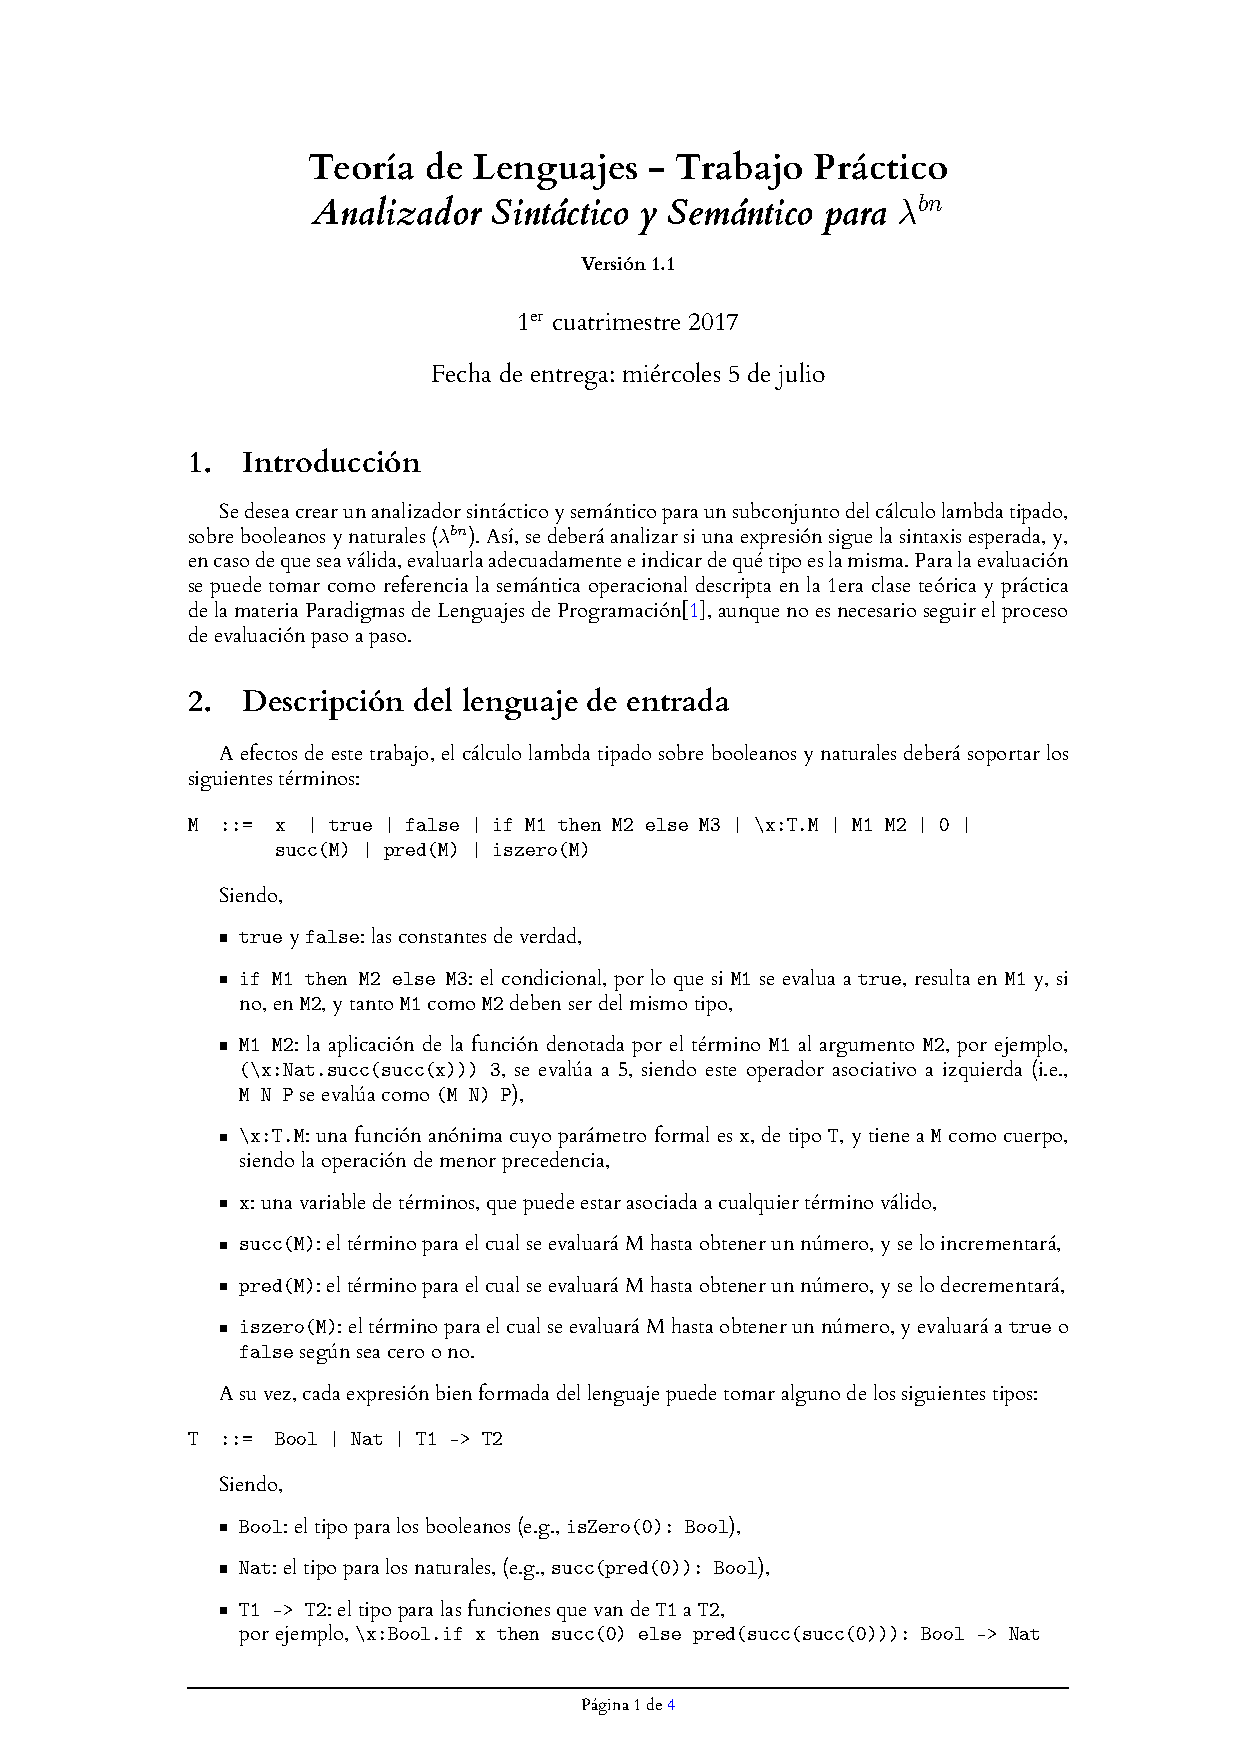
\includepdf[pages={1},pagecommand=\section{Enunciado},offset=40 -75]{enunciado.pdf}
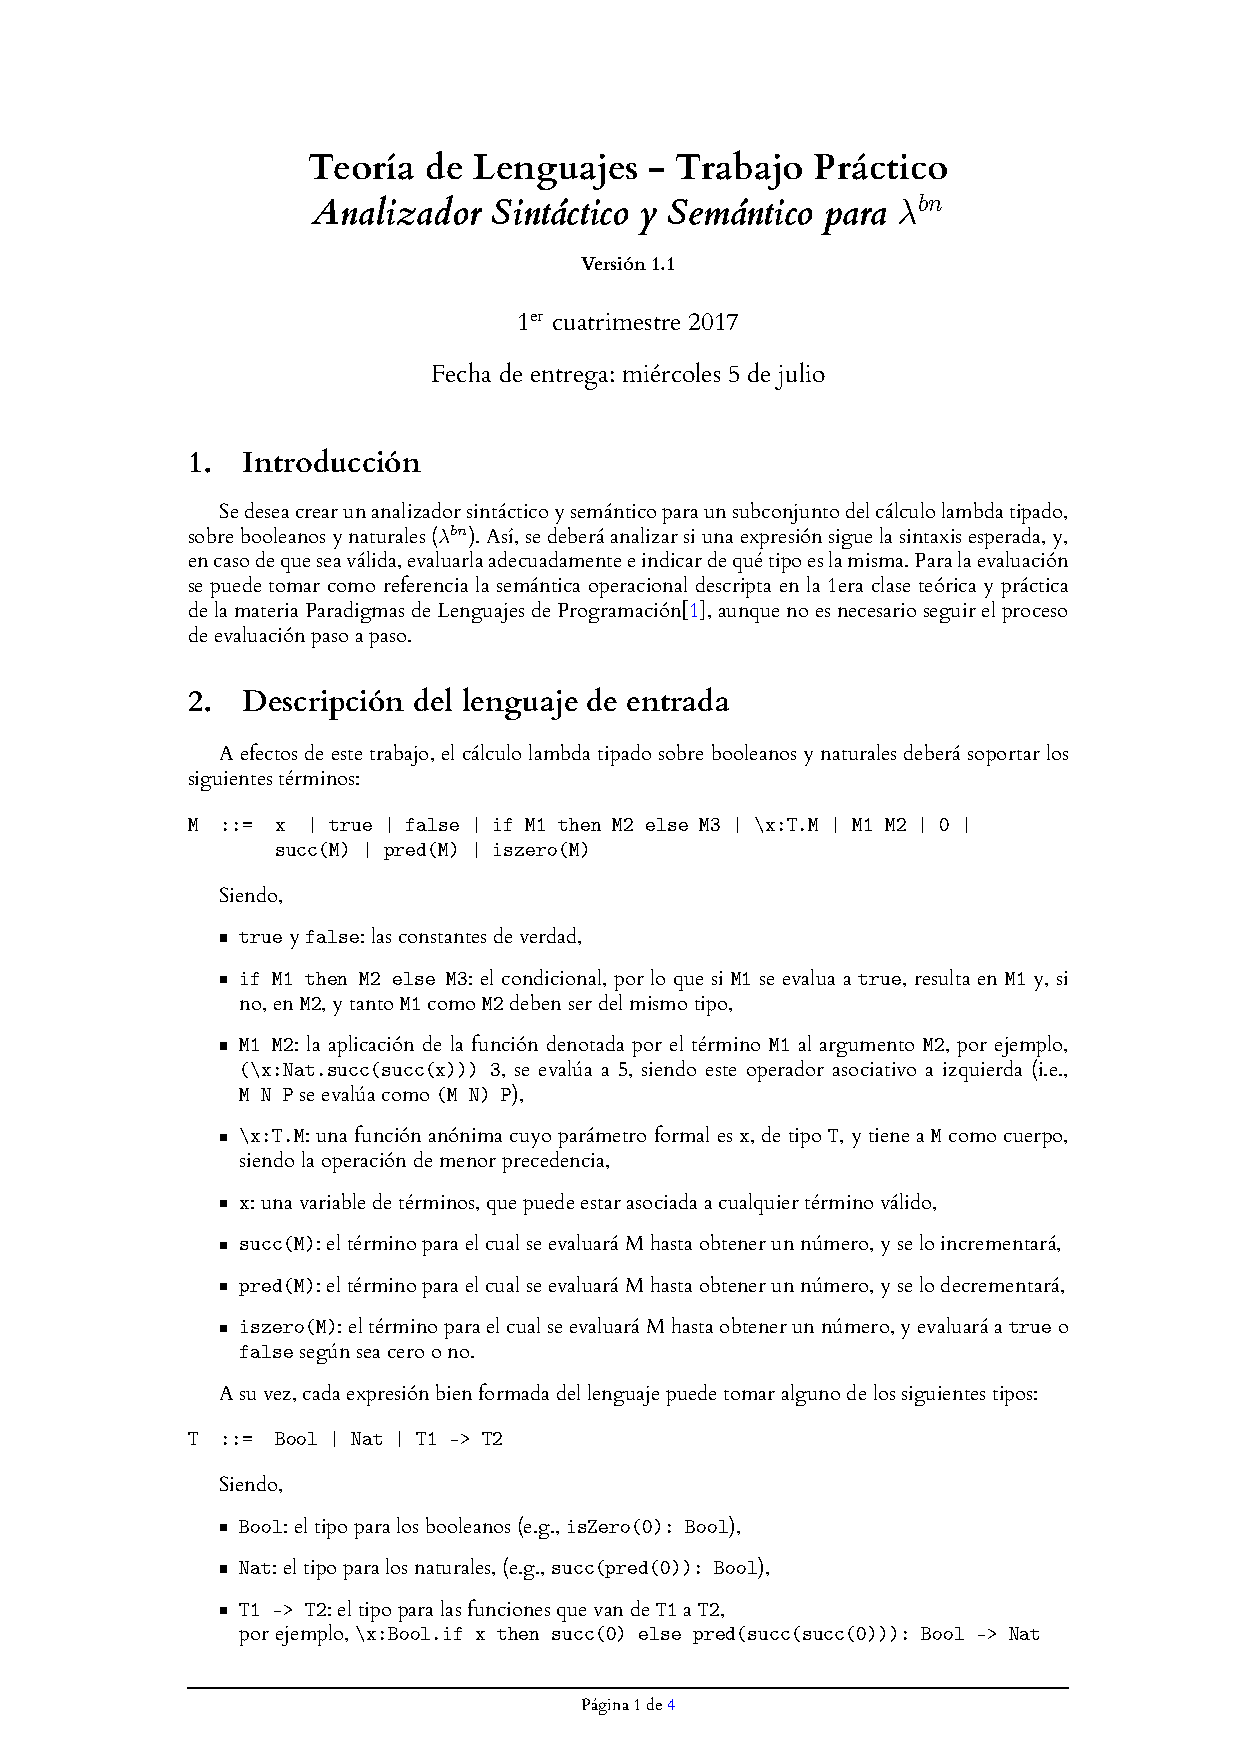
\includepdf[pages={1,2,3,4},offset=40 -75]{enunciado.pdf}

\end{document}
